%!TEX root = informe.tex
\chapter{Análisis de Ciclo de Vida de un adoquín: evaluación del impacto ambiental (EICV)}
%MADERA
Como define la norma UNE – EN ISO 14040:2006, “la fase de EICV es para conocer y evaluar la magnitud y cuán significativos son los impactos potenciales ambientales de un sistema del producto a través de todo el ciclo de vida del producto.”
En la EICV se hace un enfoque relativo del impacto ambiental basado en la unidad funcional. Acorde al alcance y los objetivos, tenemos datos y resultados suficientes en el ICV para realizar la EICV.
El contenido de la Evaluación del Impacto Ambiental se ajusta a lo establecido para estos estudios en el Reglamento del Real Decreto Legislativo 1/2008, de 11 de enero, por el que se aprueba el texto refundido de la Ley de Evaluación de Impacto Ambiental de Proyectos.

\section{Objetivo}
\subsection{Resultados}

Una vez creado el modelo completo del proceso de extracción de materias primas, fabricación e instalación, SimaPro genera un análisis de los datos introducidos. El método de análisis elegido es \textit{ReCiPe Endpoint (H) V1.06 / Europe ReCipe H/A}, previamente explicado en la sección \ref{sec:recipe}.

\begin{figure}[!htb]
\centering
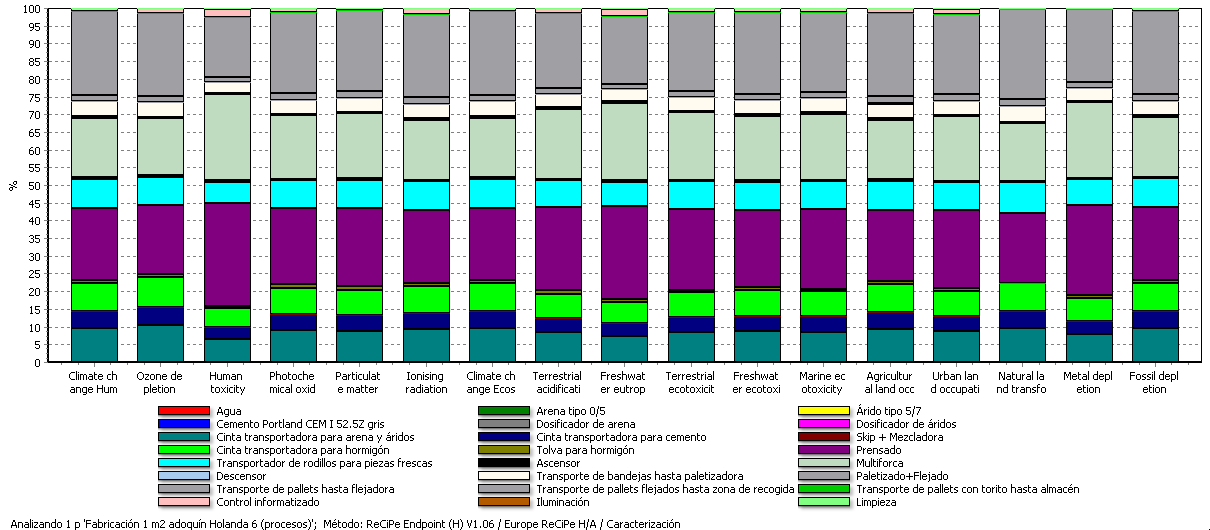
\includegraphics[angle=90,height=19cm]{img/fabricacion_caracterizacion.png}
\caption{Caracterización del análisis de fabricación de 1 \si{m^2} de adoquín.}
\label{fig:caracterizacionfabricacion}
\end{figure}

\begin{figure}[!htb]
\centering
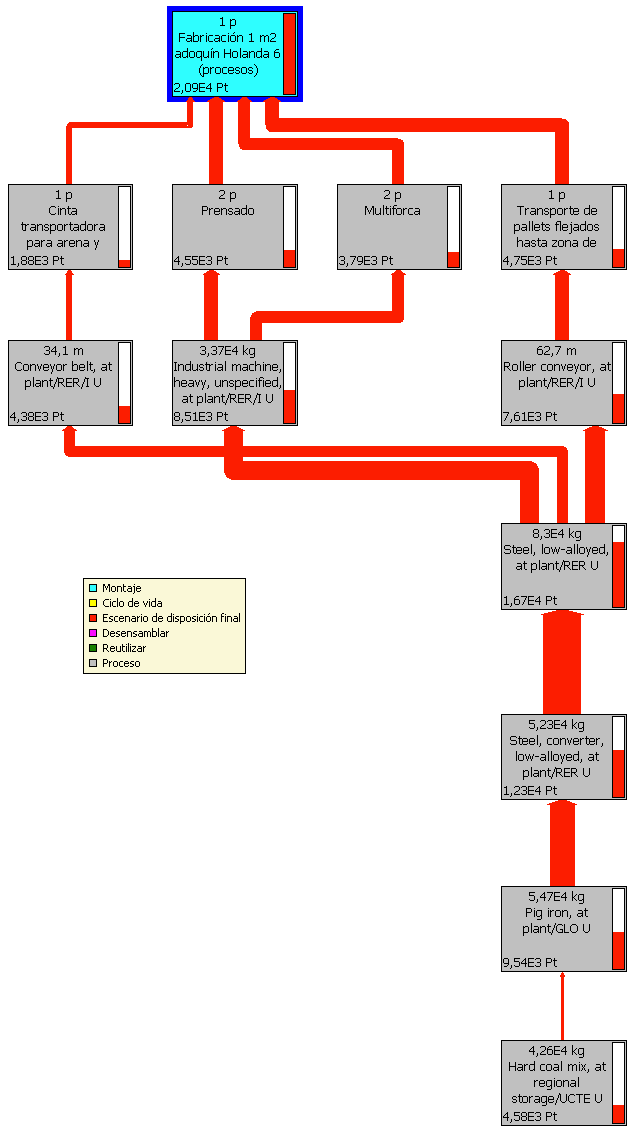
\includegraphics[height=19cm]{img/fabricacion_red.png}
\caption{Red del análisis de fabricación de 1 \si{m^2} de adoquín.}
\label{fig:redfabricacion}
\end{figure}

\section{Medidas preventivas, correctivas}
